\section{Related Work}
Diffusion Magnetic Resonance Imagining (dMRI, also referred to as Diffusion Tensor Imaging (DTI)) is a magnetic resonance imaging technique which provides three-dimensional information about the structures in cerebral white matter based on diffusion of water molecules. DTI has gained popularity in medical diagnosis within recent years, it's main clinical application is found in the study and treatment of neurological disorders. DTI may reveal abnormalities in white matter fiber structure and is used for visualizing the organization of fibers in the human brain and brain connectivity.
A variety of algorithms have been proposed for generating fiber-tract trajectories. In general, these reconstructions of fiber trajectories are clustered into bundles which are expected to be related anatomically or spatially. 
We broadly divide the related work on DTI into two parts of immediate relevance to our proposed solution: fiber tracking and fiber clustering. We next review methods for analyzing the second order local structure and the current state of the art in the visual analysis of fiber reinforced composites.
\subsection {Fiber Tracking in Diffusion Tensor Imaging}
\label{subsec:fiberEx} 
A basic assumption in DTI analysis is that the principal eigenvector of the diffusion tensor is parallel to the underlying dominant fiber direction in each image voxel~\cite{Basser2002, Mori1999, Mori2002}. The principal diffusion direction at each discrete location is interpolated to form a continuous velocity field. Continuous tracts are generated by propagating virtual particles along the principal diffusion directions until they reach some termination criterion. 
This is usually done by solving a Runge-Kutta integration (typically second or fourth order).
Because decisions are made locally, these methods perform poorly in noisy regions and often generate small fibers. Basser et al.~\cite{Basser2000,Basser2002} proposed that white matter tracts could be represented as 3D curves in space. They showed that numerical methods could be used to follow fibers and fiber bundles and to generate tracts in human brain data. 
Mori et al.~\cite{Mori1999,Mori2002} divided reconstruction techniques into line-propagation or energy minimization techniques. In line propagation approaches, trajectories are computed based on local neighborhoods and in energy minimization approaches the most favorable trajectory connecting two given endpoints is selected. 


\subsection {Fiber Clustering in Diffusion Tensor Imaging}
\label {subsec:fiberClus}
In DTI, similarity measures such as proximity between fibers are used to group fiber tracts into bundles. Extensive research has been done on automatic DTI fiber clustering methods \cite{Brun2004,Brun2003,Corouge2004,westinMEDIA02,Zhang2008}.These approaches build on the assumption that proximity measures that compare DTI fiber trajectories can also represent anatomical relationships.
Clustering requires choosing a suitable proximity measure and a method for grouping ``close" fibers.

Pairwise proximity measures include endpoint distances~\cite{Brun2003} and mean of the closest distances between points on two fibers~\cite{Corouge2004}. Zhang et al.~\cite{Zhang2008} introduced a thresholded version of the closest distances mean, so that fibers which are close for certain distance and then diverge, are clustered separately. Brun et al.~\cite{Brun2004} use normalized cuts along with a pairwise distances measure computed using a 9D fiber shape descriptors. 

The choice of the clustering algorithm can be broadly divided into those approaches using hierarchical clustering~\cite{Moberts2005, Zhang2008} and those using spectral clustering~\cite{Brun2004,jonasson2005, ODonnell2007}.
Brun et al.~\cite{Brun2003} described how a spectral non-linear dimensionality reduction technique, Laplacian eigenmaps (Belkin and Niyogi~\cite{Belkin01}), can be applied to the problem of organizing fiber tracts data. The key notion of the Laplacian eigenmaps algorithm is to represent the underlying data as a graph. Each node represents a data point and the edges connect neighboring data points. An eigenvalue problem is solved to represent the data in a lower dimensional space while preserving the local graph structure. In the case of fiber bundles, the individual points are fiber tracts. In the ideal case fiber tracts belonging to the same bundle must remain ``close" to each other in the lower dimensional space. Westin et al.~\cite{westinMEDIA02} also used spectral clustering on a Hausdorff distance measure defined as the maximum of point wise minimum distances between two fibers. Jonasson et al.~\cite{jonasson2005} ran k-means clustering on the eigenvectors of the affinity matrix defined as the co-occurrence of fibers in the data.
Additionally, the agglomerative hierarchical clustering method~\cite{DudaHartStork01} has gained popularity for proximity based fiber segregation (Zhang et al.~\cite{Zhang2008}, Corouge et al.~\cite{Corouge2004}). 
An agglomerative hierarchical clustering method starts with each data point/fiber in an individual cluster. At each stage of the algorithm the two most similar clusters are merged based on some criterion. The two basic cluster similarity measures are single-link and complete-link. With the single link, the distance between the clusters is the distance between the closest pair of items. 
Moberts et al.~\cite{Moberts2005} implemented several distance measures in their evaluation of fiber clustering and concluded that clustering methods are generally accurate in capturing fiber bundles. 
 
There are a number of difficulties in hierarchical clustering. First, computing all pairs' distances for tracts to generate the distance matrix is time consuming~\cite{Garyfallidis2012}. Second, a ``correct'' distance measure to compare tracts must be chosen. Third, hierarchical clustering is best suited for similar length fibers.
Spectral methods are also hindered by long matrix computations.


\subsection{Second order local structure}
Unlike DTI, we do not have diffusion tensor data. Instead, we have a scalar volume with tubular structures embedded in them. Analyzing curvilinear structures in volumetric images has been utilized for a variety of purposes including center line extraction~\cite{Bouix2005} and vascular image enhancement as proposed by Frangi et al.~\cite{Frangi1998} and Sato et al.~\cite{Sato1997}. Frangi et al.~\cite{Frangi1998} introduced a method based on studying the eigenvalues of the Hessian matrix specifically for the purposes of developing vessel enhancement filters.

\subsection {Visual Analysis and Modeling of Fiber Reinforced Composites}
The approaches presented in visualization and analysis of composites mainly focuses on individual objects such as fiber extraction from high resolution data where the individual fibers are clearly discernible. Fritz et al.~\cite{Fritz2009} proposed interactive workflows for non destructive testing practitioners to explore and quantify steel fibers in reinforced sprayed concrete. %This approach allows analyzing fiber orientations based on direction transfer functions. 
Salaberger et al.~\cite{Salaberger2011} introduced a pipeline to extract and characterize individual fibers of fiber reinforced composites. They encode the extracted fibers as color-coded line segments in 3D and visually identifying fibers with similar orientations.
Recently, Weissenbock et al.~\cite{Weissenbock2014} introduced a system for interactive exploration and analysis of fibers in fiber reinforced polymers. 
Lomov et al.~\cite{Lomov2010} discusses the problems and current available solutions in geometric modeling of three dimensional composites.
Modeling of the composites, first starts with establishing the topology of the structure, which translates to answering if a particular bundle is in contact with another at a particular position? The second step builds the geometry of the model, answering queries relating to placement of bundles in space, their orientations and dimensions. 
\begin{figure}[htb]
\centering
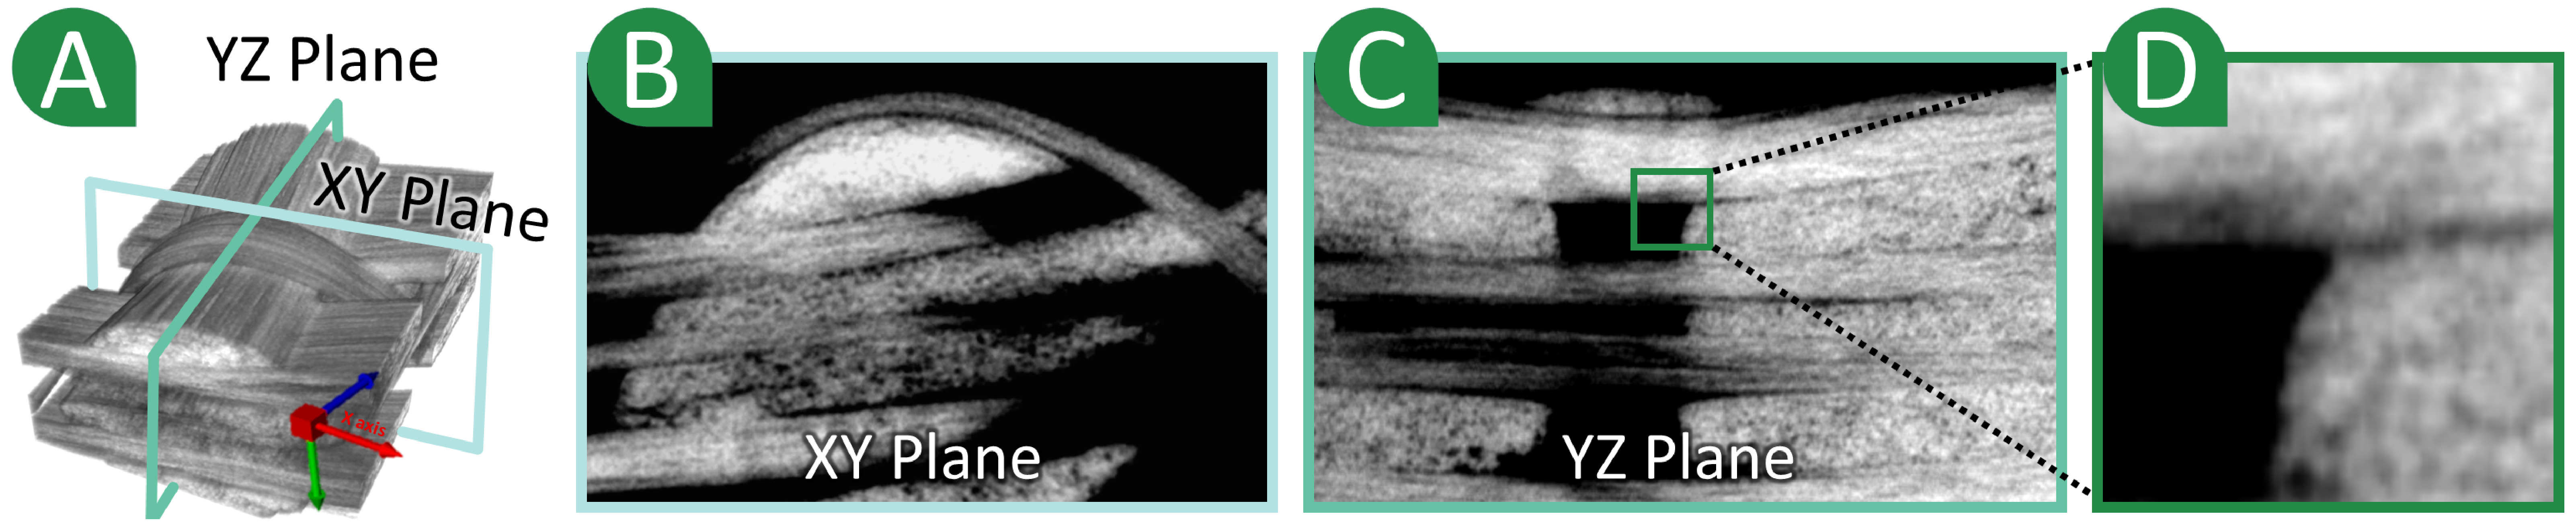
\includegraphics[width=\linewidth]{images/data-char.eps}
\caption
{
Data characteristics: (a) Rendering of dataset D1. (b, c) 2D slices along Z- and X-axis. (d) Zoom in of the green region marked in (c). Multiple fiber bundles cross and are indistinguishable by visual inspection alone. 
}
\label{fig:data-char}
\end{figure}

\section {Data Characteristic and Assumptions}
\label{sec:char_data}
Figure~\ref{fig:data-char} shows dataset D1 with woven fiber bundles. The size of D1 is 450$\times$300$\times$500 voxels with isotropic resolution of 2 $\mu m$ and 8 bit unsigned integer scalars. Figure~\ref{fig:data-char} clearly shows the recurring fiber bundle weaving pattern of the composite unit cell used for manufacturing fiber composites. Figure~\ref{fig:data-char}\brac{a} shows a volume rendering of the dataset. Figure~\ref{fig:data-char}\brac{b} and ~\ref{fig:data-char}\brac{c} show 2D slices along the $X$- and the $Z$-axis respectively. Figure~\ref{fig:data-char}d zooms into the green region of interest. 
Figure~\ref{fig:data-char}\brac{d} contains two bundles going in opposite directions, the low resolution of D1 renders the individual carbon fibers in a fiber bundle hard to resolve. Also the separation between two fiber bundles is barely visible. The fiber bundles may differ in terms of the amount of fibers in the bundle. Figure~\ref{fig:data-char}\brac{a} shows the large variation in cross section sizes among the bundles.
Depending on the weaving pattern, the fiber bundles cross each other in different orientations. The number of orientations is defined by the weaving pattern and typically consists of two main orientations. The weaving pattern may cause individual bundles to be curved. In consequence, individual fibers may be adjacent in Euclidean distance but belong to different bundles. 
We make the following \textit{assumptions} on our data:

\begin{itemize}[noitemsep]
\item The structure embedded in the data contains fiber bundles of indiscernible fibers.
\item Local orientation: each point in a fiber bundle has a local orientation parallel to the corresponding area in the fiber bundle.
\item Local orientation may gradually change within the fiber bundle.
\item Local orientation may be noisy and not reliable.
\item Connectivity: moving along the direction of a non-noisy local orientation in small increments, we will reach another neighborhood with similar local orientation.
\item Fiber bundles going in different directions only interact near the surface of contact.
\end{itemize}